\begin{SCfigure}[][htbp]

% \begin{center}
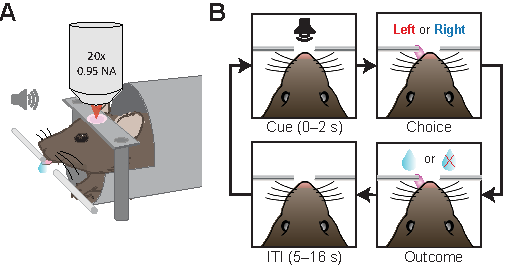
\includegraphics[width=8.7cm]{Figures/Introduction/Intro_fig_ExpSetup} 
% \end{center}
\caption[Experimental framework]
{Common experimental framework for the experiments presented in Chapters 1--3. (A) Experimental apparatus for dual-choice auditory-motor task with simultaneous two-photon imaging. (B) Flow diagram of trial structure. A sound cue was played at the start of each trial, indicating the target spout that would be rewarded (left or right). To obtain the reward, subjects were required to lick the target within 2 s following cue onset. After an intertrial interval (ITI) of 5--16 s, a new sound cue was presented, providing a fresh opportunity to lick for a reward. }


\label{fig:Intro_ExpSetup}
\end{SCfigure}
